%%
% Please see https://bitbucket.org/rivanvx/beamer/wiki/Home for obtaining beamer.
%%



\documentclass[hyperref={pdfpagelabels=false},xcolor=dvipsnames]{beamer}
\usepackage{lmodern}
%\mode<presentation>{
%\usetheme{Copenhagen}
\usecolortheme{dove}
\setbeamertemplate{footline}[page number]
%\setbeamertemplate{navigation symbols}{}
%}

\usetheme{Singapore}
%\usecolortheme[named=Gray]{structure}
\usepackage[utf8]{inputenc}
\usepackage[ngerman]{babel}
\usepackage{graphicx}
%\usepackage{booktabs}
\setbeamertemplate{navigation symbols}{}




\setbeamercolor{normal text}{fg=darkgray}
\setbeamercolor{frametitle}{fg=darkgray}

\setbeamercolor{title}{fg=darkgray}

\setbeamercolor{titlelike}{fg=darkgray}
%\setbeamercolor{tableofcontents}{fg=red}

%\setbeamercolor{background canvas}{use={titlelike},bg=gray}

\usebeamercolor*{normal text}
\usebeamercolor*{frametitle}

\usebeamercolor*{title}
%\usebeamercolor*{tableofcontents}



\newcommand*\mi{ \item[\color{gray}\scalebox{1.2}{\textbullet}]}


\title{VLAN und VPN}
\author{KL}
\institute{Fernuniversität Hagen}
\date{WS 18/19}





\begin{document}

\begin{frame}[plain]
	\titlepage
\end{frame}
%%%%%%%%%%%
\begin{frame}[plain]

	\frametitle{Inhalt}
	\tableofcontents	
\end{frame}
%%%%%%%%%%%
\section{Einleitung}

\begin{frame}
	\frametitle{IT-Sicherheit in kleinen Unternehmen} Studie des WIK: 	
	\begin{itemize}
		\mi 64\% der kleinen Unternehmen finden IT-Sicherheit sehr wichtig
		\mi $20\%$ haben eine Sicherheitsanalyse durchgeführt
		\mi $94\%$ haben PC-Arbeitsplätze mit Internetzugang
		\mi $75\%$ nutzen mobile Endgeräte (Smartphone, Tablet, Notebook)
		\mi 31\% nutzen VPN
		\mi 53\%	waren von Virenangriffen betroffen
	\end{itemize}
	
\end{frame}
%%%%%%%%%%%
\section{Sichere Netzwerkarchitektur}
\begin{frame}
\sectionpage	
\end{frame}


\begin{frame}
	\frametitle{Grundarchitektur eines sicheren Netzwerkes}
	\begin{figure}
	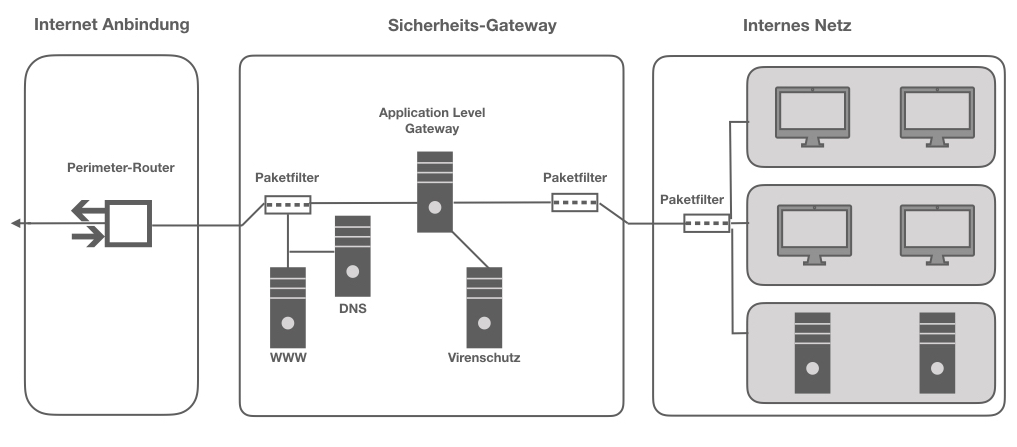
\includegraphics[width=\textwidth]{grundarchitektur.jpeg}	
	\end{figure}
		
\end{frame}
%%%%%%%%%%%%
\begin{frame}

	\frametitle{Grundarchitektur für kleine Unternehmen}
	\begin{columns}
		\column{.5\textwidth}
		\centering Hoher Schutzbedarf
				\begin{figure}
				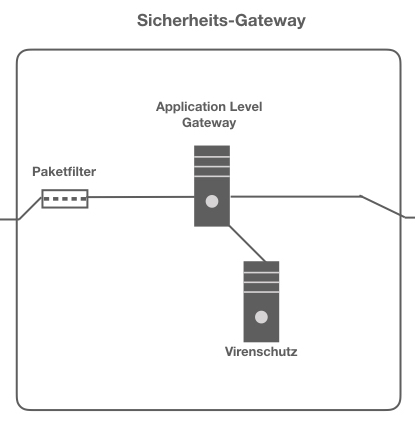
\includegraphics[width=.8\textwidth]	{arch.001.jpeg}
			\end{figure}
	
		\column{.5\textwidth}
		\centering Normaler Schutzbedarf
		\begin{figure}
			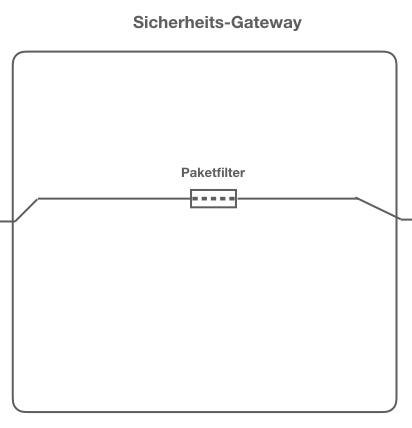
\includegraphics[width=.8\textwidth]	{arch.002.jpeg}
		\end{figure}
	\end{columns}	
\end{frame}



%%%%%%%%%%%%%%
%%%%%%%%%%%%%%
\section{Virtuelle lokale Netzwerke VLAN}
%%
\frame{\sectionpage}
%%
\begin{frame}
	\frametitle{Virtuelle lokale Netze VLAN}
	\begin{itemize}
		\mi  physische LANs in logische Einheiten unterteilen
		\mi verschiedene physische Netze virtuell zu verbinden
		\mi Kostenersparnis $\leftarrow$ weniger Hardware
		\mi Hohe Flexibilität
		\mi Verkleinerung der Broadcastdomäne
		 
		
	\end{itemize}

\end{frame}

%%%%%%%%%%%%%%
\begin{frame}

	\frametitle{Portbasiertes VLAN}
	
	\begin{figure}
	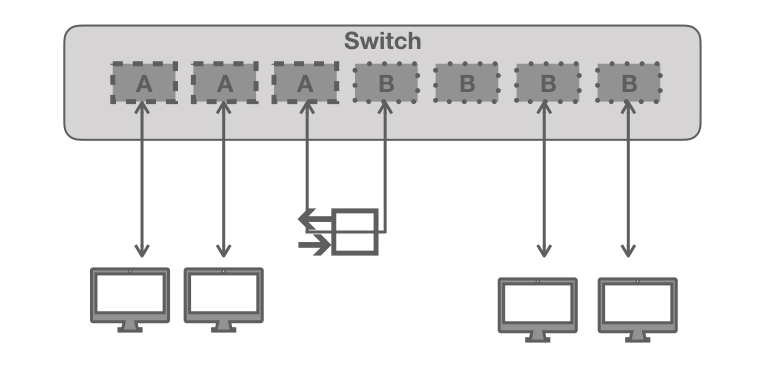
\includegraphics[width=\textwidth]{vlan.001.jpeg}	
	\end{figure}
		
\end{frame}

%%%%%%%%%%%%%%%
\begin{frame}
	\frametitle{Tagged VLAN}
		\begin{figure}
	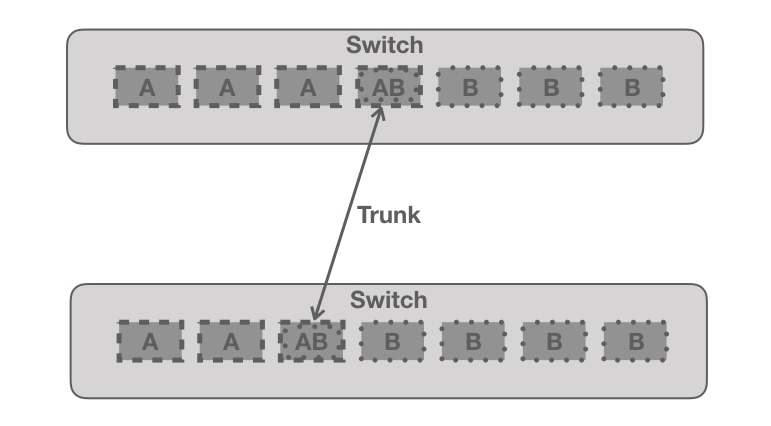
\includegraphics[width=\textwidth]{vlan.002.jpeg}	
	\end{figure}	
\end{frame}

%%%%%%%%%%%%%%%%

\begin{frame}
	\frametitle{Dynamisches vs Statiches VLAN}
	Statische VLAN
	\begin{itemize}
		\mi feste Zuordnung von Ports zu einem VLAN
		\mi Änderungen müssen manuell von Administrator vorgenommen werden 
		\mi relativ sicher	
	\end{itemize}
	Dynamisches VLAN
	\begin{itemize}
		\mi Zuordnung zum VLAN anhand von MAC- oder IP-Adressen
		\mi Flexibel
		\mi Manipulationsgefahr
		
			
	\end{itemize}

\textbf{Das BSI rät  ausdrücklich von der Nutzung dynamischer VLANs ab!}
	
\end{frame}

%%%%%%%%%%%%%%%
\begin{frame}
	\frametitle{In der Praxis zu konfigurierende VLANs}	
	\begin{itemize}
		\mi Default VLAN: auf Switch voreingestellt
		\mi Data VLAN: Netzwerk für Endgeräten
		\mi Native VLAN: ungetaggte Frames die über einen Trunk geschickt werden, werden diesem VLAN zugeordnet
		\mi Management VLAN: nur von diesem sollte die Switchkonfiguration möglich sein
		\mi VoIP VLAN: VLAN für VoIP-Telefone 	
	\end{itemize}

	
\end{frame}


%%%%%%%%%%%%%%%

\begin{frame}
	\frametitle{VLAN und Sicherheit}
	\begin{block}{BSI}
	\glqq Entgegen den Aussagen einiger Hersteller muss berücksichtigt werden, dass VLANs nicht entwickelt wurden, um Sicherheitsanforderungen bei der Trennung von Netzen zu erfüllen.\grqq 
	\end{block}
	
	\begin{block}{Bedrohungen}
		\begin{itemize}
			\mi VLAN Hopping: double tagging /switch spoofing 	
			\mi MAC-Flooding
		\end{itemize}
	\end{block}
	
	\begin{block}{Vorteil}
		Trotzdem ist ein gut konfiguriertes VLAN eine zusätzliche Hürde für einen Angreifer. 
	\end{block}



\end{frame}

%%%%%%%%%%%%%
%%%%%%%%%%%%%
\section{Virtuelle Private Netze VPN}
%%
\frame{\sectionpage}


%%
\begin{frame}
	\frametitle{VPN Varianten}
	\begin{itemize}
		\mi Site-to-Site/ Branch Office VPN: Verbindung von Firmenstandorten
		\mi End-to-Site/Remote Access: Heimarbeitsplatz, Mobiler Mitarbeiter
		\mi End-to-End: Verbindung zweier Endgeräte
		\mi Extranet VPN: Zugang für Geschäftspartner/Kunden	
	\end{itemize}

\end{frame}
%%%%%%%%%%%%%
%\subsection{Tunneling}
%%%%%%%%%%%

\begin{frame}
	\frametitle{Tunneling}
	\begin{figure}
		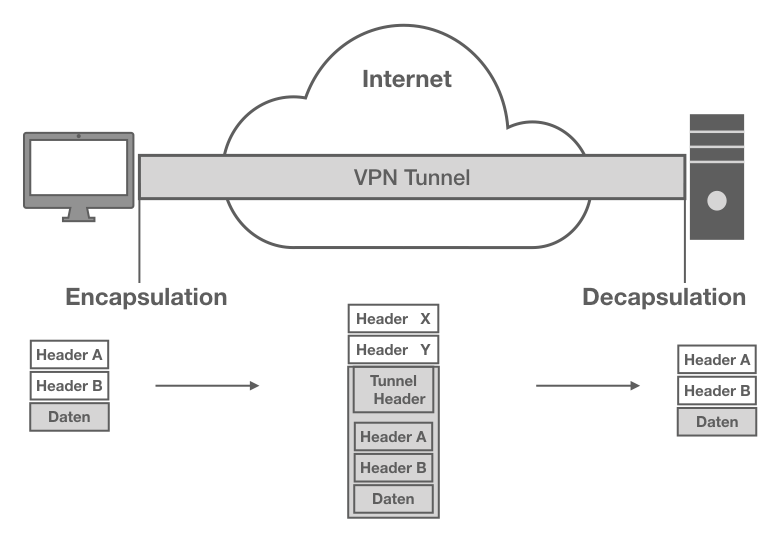
\includegraphics[width=0.8\textwidth]{tunneling}	
	\end{figure}
\end{frame}

%%%%%%%%%%%%
\begin{frame}
	\frametitle{Tunneling auf verschiedenen Schichten}
	\begin{columns}
		\column{.3\textwidth}
		\centering Hybridmodell OSI - TCP/IP: 
		\begin{figure}
			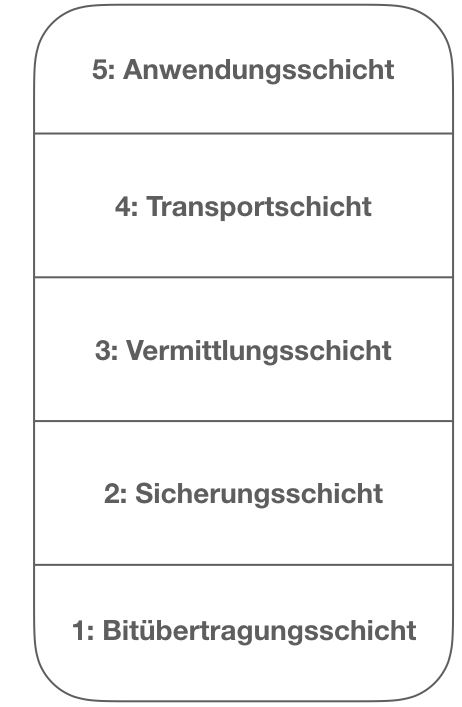
\includegraphics[width=\textwidth]{schichten.001.jpeg} 	
		\end{figure}

		\column{.7\textwidth}
		\begin{itemize}
			\mi Tunneling kann theoretisch auf jeder Schicht stattfinden
			\mi VPNs auf niedrigen Schichten sind sehr flexibel 
			\mi VPN auf Layer 3 kann sich die IP-Struktur zu nutze machen
				
		\end{itemize}
	
		
	\end{columns}

		
\end{frame}

%%%%%%%%%%%%
\begin{frame}
	\frametitle{Layer 3 Tunneling: IPSec }
	Zum Internet Security Protokoll gehören
	\begin{itemize}
		\mi	Internet Key Exchange (IKEv2): Schlüsselaustausch, Authentisierungsverfahren 
		\mi Authentication Header (AH): Authentizität, Integrität
		\mi Encapsulating
Security Payload (ESP): Authentizität, Integrität, Vertraulichkeit
		
	\end{itemize}	
\end{frame}

%%%%%%%%%%%%
\begin{frame}
	\frametitle{IPSec II}
	\begin{figure}
		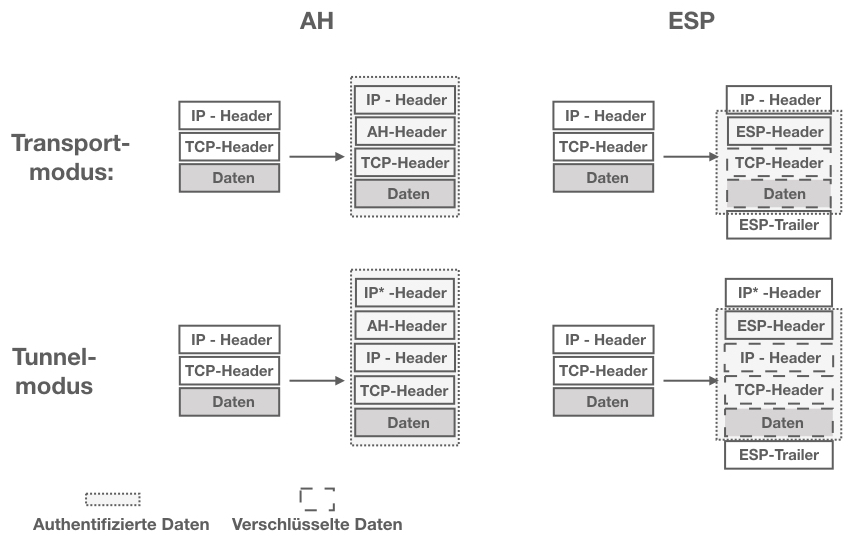
\includegraphics[width=\textwidth]{ahsep.001.jpeg}	
	\end{figure}	
\end{frame}

%%%%%%%%%%%%
\begin{frame}
	\frametitle{Layer 2 Tunneling: L2TP}
	\begin{block}{Layer 2 Tunneling Protokol}
	\begin{itemize}
		\mi kapselt Daten in Point-to-Point-Protocol (PPP) Rahmen
		\mi kann kann auch nicht-IP-Pakete über das Internet transportieren	
		\mi Extensible Authentication
Protocol (EAP) oder Challenge Handshake Protocol (CHAP), zur Authentifizierung
		\mi mehrere Verbindungen über einen Tunnel möglich
		\mi Kombination mit IPSec möglich 
		
	\end{itemize}
	\end{block}
		 
\end{frame}

%%%%%%%%%%%%
\begin{frame}
	\frametitle{Anwendungs- / Transportschicht VPN}
	\begin{itemize}
		\mi z.B. open VPN
		\mi SSL (Secure Socket Layer) / TLS (Transport Layer Security)
		\mi	verschlüsselte Verbindungen ohne Tunnel werden auch als SSL-VPN bezeichnet
		\mi auch mit Tunnel möglich, z.B. mit PPP Paketen
	\end{itemize}

		 
\end{frame}

%%%%%%%%%%%%
\begin{frame}
	\frametitle{Einbindung des VPN-Gateways in das Sicherheits-Gateway}
	\begin{figure}
		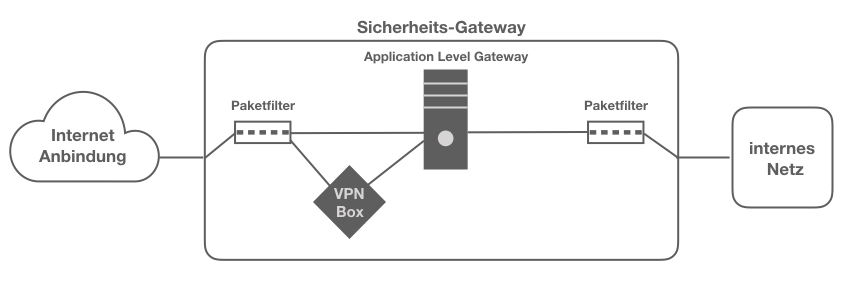
\includegraphics[width=\textwidth]{vpnarchitektur.jpeg}	
	\end{figure}	
	\begin{itemize}
		\mi vor Angriffen aus dem Internet geschützt
		\mi eingehende Kommunikation kann vom ALG überprüft werden	
	\end{itemize}

	
\end{frame}
%%%%%%%%%%%%%%
\begin{frame}
	\frametitle{Private Nutzung von VPN}
	\begin{itemize}
		\mi Zugriff auf das Heimnetz (z.B IoT, NAS)
		\mi Sicheres Surfen in offenen WLANs
		\mi Überwinden von Geoblocking, anonymes Surfen	
	\end{itemize}

	\begin{figure}
		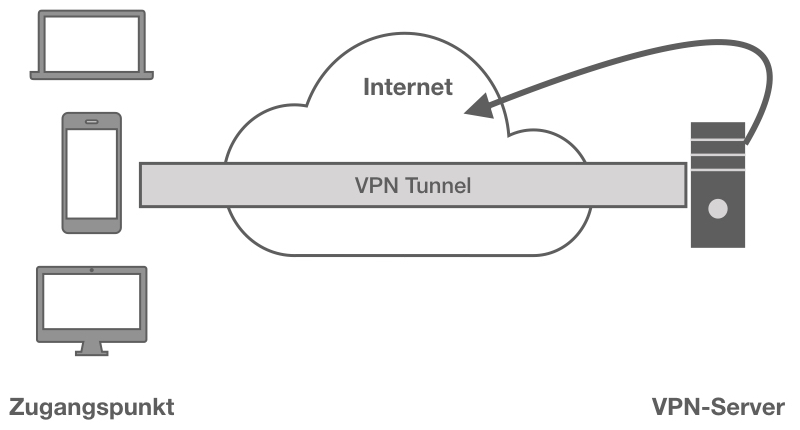
\includegraphics[width=.9\textwidth]{vpnPrivat.001.jpeg}	
	\end{figure}

		 
\end{frame}

%%%%%%%%%%%%%
%%%%%%%%%%%
\section{Ausblick}

\begin{frame}
	\frametitle{Ausblick}
	\begin{itemize}
		\mi Security by Design: Sicherheit nicht als Option sonder als Teil des Netzwerks!
		\mi SDN (Software defined Networking): Netzwerke der Zukunft?
		
	\end{itemize}	
\end{frame}


\end{document}



